\chapter{Implementacija i korisničko sučelje}
		
		
		\section{Korištene tehnologije i alati}
		
			\textbf{\textit{dio 2. revizije}}
			
			Backend dio aplikacije pisan je u objektno orijentiranom programskom jeziku  \href{https://www.java.com/en/}{\textbf{Java}}\footnote{https://www.java.com/en/}. Jedna od glavnih značajki ovog jezika je takozvano načelo WORA (eng. \textit{write once, run anywhere}) koje omogućava da se jednom prevedeni kod pomoću Javinog virtualnog stroja može izvršavati na bilo kojem računalu. Jedini preduvjet je da to računalo na sebi ima instaliranu Javinu platformu.
			
			Kako bi se olakšao razvoj backend dijela aplikacije, korišten je radni okvir \href{https://spring.io/projects/spring-boot/}{\textbf{Spring Boot}}\footnote{https://spring.io/projects/spring-boot/} koji je specijalizacija radnog okvira Spring. Spring Boot je popularan radni okvir za izgradnju samostojećih web aplikacija. Glavna prednost ovog radnog okvira je automatska konfiguracija dijelova koda koji se standardno pojavljuju kod web aplikacija. Tako Spring Boot automatizira komunikaciju s bazom podataka, rad s datotekama u JSON formatu, podjela programskog koda u unaprijed definirane slojeve itd.
			
			Backend dio aplikacije je razvijan u razvojnom okruženju \href{https://www.jetbrains.com/idea/}{\textbf{IntelliJ IDEA}}\footnote{https://www.jetbrains.com/idea/} tvrtke JetBrains. Samo razvojno okruženje je namjenjenu razvoju u programskim jezicima Java, Kotlin, Groovy, Scala te je jedno od vodećih okruženja za te programske jezike. IntelliJ IDEA programeru nudi razne funkcionalnosti koje ubrzavaju i olakšavaju programiranje kao što su samozavršavanjne koda analizom konteksta, navigacija u kodu, refaktoriranje koda, debuggiranje, rad sa distribuiranim sustavima za upravljanje verzijama podataka, kao što je Git, rad s bazom podataka itd. Također, IntelliJ IDEA programer može dodatno nadograditi instaliranjem proširenja za dodatne funkcionalnosti koja su dostupna na web repozitoriju JetBrainsa.
			
			Frontend dio aplikacije je pisan u programskom jeziku \href{https://www.javascript.com/}{\textbf{JavaScript}}\footnote{https://www.javascript.com/} koji efektivno postao nezabiolazan jezik za razvoj klijentske strane web aplikacija. JavaScript je dinamičan skriptni jezik sa mekim tipovima podataka (eng. \textit{soft-typed}) kojeg podržava svaki moderan web preglednik. Za sam jezik JavaScript postoji napisano puno javno dostupnih biblioteka koje olakšavaju ostvarivanje raznih funkcionalnosti u kodu i potiču ponovnu uporabu postojećeg koda. Iako je Javascript de facto standard za razvoj frontend dijela aplikacije, također se može koristiti i za razvoj backend dijela aplikacije.
			
			Za brži i lakši razvoj frontend dijela aplikacije korištena je vrlo popularna biblioteka  \href{https://react.dev/}{\textbf{React}}\footnote{https://react.dev/} razvijena od tvrtke Meta (nekada Facebook). Aplikacije napravljene u Reactu koriste komponente koje se mogu koristiti na više mjesta. React koristi virtualni DOM (Document Object Model) te se pomoću Reacta grade jednostranične web aplikacije koje osvježavaju samo komponente koje je potrebno mijenjati. Time se značajno poboljšavaju performanse web aplikacije.
			
			Kako bi dodatno olakšali vizualno oblikovanje korisničkog sučelja korišten je radni okvir \href{https://getbootstrap.com/}{\textbf{Bootstrap}}\footnote{https://getbootstrap.com/}. Bootstrap je popularan radni okvir za stilski jezik CSS koji olakšava vizualno oblikovanje korisničkog sučelja nuđenjem gotovih dizajnova osnovnih elemenata web stranice kao što su na primjer gumbovi, forme i sl. 
			
			Za razvoj frontend dijela aplikacije korišteno je razvojno okruženje \href{https://code.visualstudio.com/}{\textbf{Visual Studio Code}}\footnote{https://code.visualstudio.com/} tvrtke Microsoft. Visual Studio Code je moguće nadograđivati raznim proširenjima pomoću kojih se može stvoriti razvojno okruženje za gotovo svaki programski jezik kao što je C, C++, Java, JavaScript, Python, Go, itd. Zbog te fleksibilnosti se Visual Studio Code može koristiti u gotovo svakoj domeni koja uključuje neku vrstu programiranja.
			
			Baza podataka je napravljena u sustavu \href{https://www.postgresql.org/}{\textbf{PostgreSQL}}\footnote{https://www.postgresql.org/}. PostgreSQL je jedan od najraširenijih sustava za upravljanje relacijskim bazama podataka temeljen na SQL-u (Structured Query Language). PostgreSQL omogućuje izradu baza podataka sa raznim funkcionalnostima kao što su okidači, transakcije, procedure, mogćnost paralelnog pristupa više korisnika istovremeno, konzistencija i sigurnost podataka, itd.
			
			Svi dijagrami za opis sustava napravljeni su u \href{https://www.uml.org/}{\textbf{UML-u}}\footnote{https://www.uml.org/} (Unified Modeling Language). UML je generički jezik za vizualno modeliranje. Napravljen je kako bi pružao standard za dizajniranje sustava. Taj standard omogućava bolju vizualizaciju, specifikaciju, oblikovanje i dokumentiranje artefakata programske potpore. U svrhu vizualizacije pojedinog aspekta sustava definiran je veliki broj vrsta dijagrama koji omogućuju različite poglede na pojedini dio sustava.
			
			Za izradu UML dijagrama korišten je grafički alat \href{https://www.visual-paradigm.com/}{\textbf{Visual Paradigm}}\footnote{https://www.visual-paradigm.com/}. On podržava izradu mnogih vrsta UML dijagrama kao što su dijagram obrazaca uporabe, sekvencijski dijagram, dijagram stanja, dijagram komponenti, dijagram aktivnosti, dijagram razmještaja, dijagram razreda, i mnogi drugi.
			
			Za potrebe izrade dijagrama razreda korištena je funkcionalnost razvojnog okruženja IntelliJ IDEA za automatsko generiranje dijagrama razreda iz postojećeg programskog koda. Dobiveni dijagram razreda je dodatno uređen i dorađen u grafičkom alatu za izradu dijagrama  \href{https://www.drawio.com/}{\textbf{draw.io}}\footnote{https://www.drawio.com/}.
			
			Izrada relacijskog dijagrama baze podataka i modeliranje same baze podataka ostvareno je uz grafički alat \href{https://erdplus.com/}{\textbf{ERDPlus}}\footnote{https://erdplus.com/}. ERDPlus omogućuje izradu ER dijagrama baze podataka koji se sastoji od entiteta i veza između njih. Iz ER dijagrama je moguće automatsko generiranje relacijskih dijagrama baze podataka. Iz dobivenih relacijskih dijagrama je moguće automatsko generiranje SQL naredbi za stvaranje odgovarajućih tablica u bazi podataka.
			
			Dokumentacija je pisana u jeziku \href{https://www.latex-project.org/}{\textbf{LaTeX}}\footnote{https://www.latex-project.org/}. LaTeX je široko korišten jezik za pisanje dokumenata koji pruža široke mogućnosti i omogućuje jednostavniju izradu složenih dokumenata. S obzirom da se radi o markup jeziku, LaTeX omogućuje odvajanje stila od sadržaja što kod složenih dokumenata daje veliku prednost u odnosu na standardne aplikacije za pisanje dokumenata kao što su MS Word.
			
			U svrhu pisanja dokumentacije u LaTeX-u korišten je \href{https://www.texstudio.org/}{\textbf{TeXstudio}}\footnote{https://www.texstudio.org/}. TeXstudio je uređivač teksta posebno napravljen upravo za pisanje dokumenata u jeziku LaTeX.
			
			Za upravljanje programskim kodom, dokumentacijom i ostalim datotekama koje su korištene u ovom projektu korišten je sustav \href{https://git-scm.com/}{\textbf{Git}}\footnote{https://git-scm.com/}. Git je popularan distribuirani sustav za upravljanje verzijama podataka. Izuzetno je koristan kada više ljudi u timu radi na nekom projektu jer omogućuje koordinaciju istovremenog rada više ljudi na projektu. Sastoji se od udaljenog repozitorija, obično na nekoj Git platformi u oblaku, te lokalnih kopija tog repozitorija na računalima korisnika koji sudjeluju u projektu. Git prati kompletnu povijest promjena u repozitoriju i nudi razne mogućnosti koje olakšavaju distribuirani rad.
			
			Kao Git platforma u oblaku je za ovaj projekt korišten \href{https://github.com/}{\textbf{GitHub}}\footnote{https://github.com/}. GitHub je danas najraširenija platforma za spremanje programskih projekata i distribuirani sustav za upravljanje verzijama.
			
			Za puštanje aplikacije i popratne baze podataka u pogon korištena je usluga oblaka \href{https://render.com/}{\textbf{Render}}\footnote{https://render.com/}. Render je sustav u oblaku koji služi za izgradnju i pokretanje raznih programskih sustava, pa tako i web aplikacija i baza podataka. Prednosti Rendera su njegovo lagano integriranje s GitHubom, automatsko deployanje prilikom promjena na grani u Git repozitoriju te postojanje besplatne usluge uz određena ograničenja koja za ovaj projekt nisu pretjerano bitna.
			
			Prilikom puštanja web aplikaacije u pogon korištena je tehnologija \href{https://www.docker.com/}{\textbf{Docker}}\footnote{https://www.docker.com/}. Docker omogućuje jednostavnu izradu kontejnera koji u sebi sadrže neku programsku podršku. Kontejner je oblik virtualizacije na razini operacijskog sustava. Ovim oblikom virtualizacije se stvara okruženje jednostavnije od onog dobivenog virtualnim strojem, ali još uvijek omogućuje da programska podrška u kontejneru bude nezavisna od okruženja na kojem je kontejner pokrenut. Docker kontejner se opisuje posebnom skriptom koja se zove Dockerfile.  
			
			Članovi tima su međusobno komunicirali preko društvenih mreža \href{https://discord.com/}{\textbf{Discord}}\footnote{https://discord.com/} i \href{https://www.messenger.com/}{\textbf{Messenger}}\footnote{https://www.messenger.com/}. Messenger je jednostavna društvena mreža koja kao glavni način komunikacije koristi izmjenu poruka između dva korisnika ili unutar grupe korisnika. Discord je društvena mreža u kojoj korisnici mogu komunicirati porukama, glasovnim pozivima i video pozivima. Korisnici mogu komunicirati unutar širih zajednica koje se nazivaju serveri. Unutar servera postoje tekstualni kanali kao i glasovni kanali za glasovne pozive sa više korisnika.
			
			Za ispitivanje sustava u cjelini korišten je radni okvir \href{https://www.selenium.dev/}{\textbf{Selenium}}\footnote{https://www.selenium.dev/}. Selenium je alat koji služi za testiranje web aplikacija pomoću web preglednika. Skripte za testiranje se mogu pisati u raznim programskim jezicima. 
			
			Za testiranje pojedinih komponenti sustava korišten je radni okvir \href{https://junit.org/junit5/}{\textbf{JUnit}}\footnote{https://junit.org/junit5/}. JUnit je radni okvir koji služi za testiranje funkcionalnosti pojedinih dijelova programskog koda pisanog u programskom jeziku Java.
			
			\eject 
		
	
		\section{Ispitivanje programskog rješenja}
			
			\textbf{\textit{dio 2. revizije}}\\
			
			\subsection{Ispitivanje komponenti}
			
			Ispitivanje komponenti vrši se radi provjeravanja ispravnosti pojedinih klasa i metoda sustava. Testovi se izvode tako što se ispitivaoj metodi šalje neki ulaz i provjerava se ponašanje metode na dobivenu ulaz sa očekivanim.
			
			Za ispitivanje komponenti sustava koristili smo JUnit testove. Svi testovi su bili uspješni, kao što je prikazano na slici \ref{fig:JUnitTestovi}.
			
			\begin{figure}[H]
				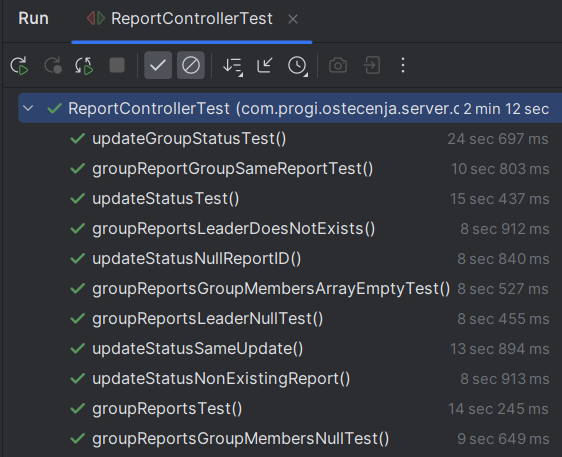
\includegraphics[width=\textwidth]{slike/JUnitTestoviRez.png} %veličina u odnosu na širinu linije
				\caption{Rezultati testova komponenti}
				\label{fig:JUnitTestovi} %label mora biti drugaciji za svaku sliku
			\end{figure}
			
			Prije svakog testa se u sustavu stvaraju dvije prijave u svrhu testiranja. Nakon svakog testa se iste prijave uklanjaju iz baze podataka.
			
			\begin{figure}[H]
				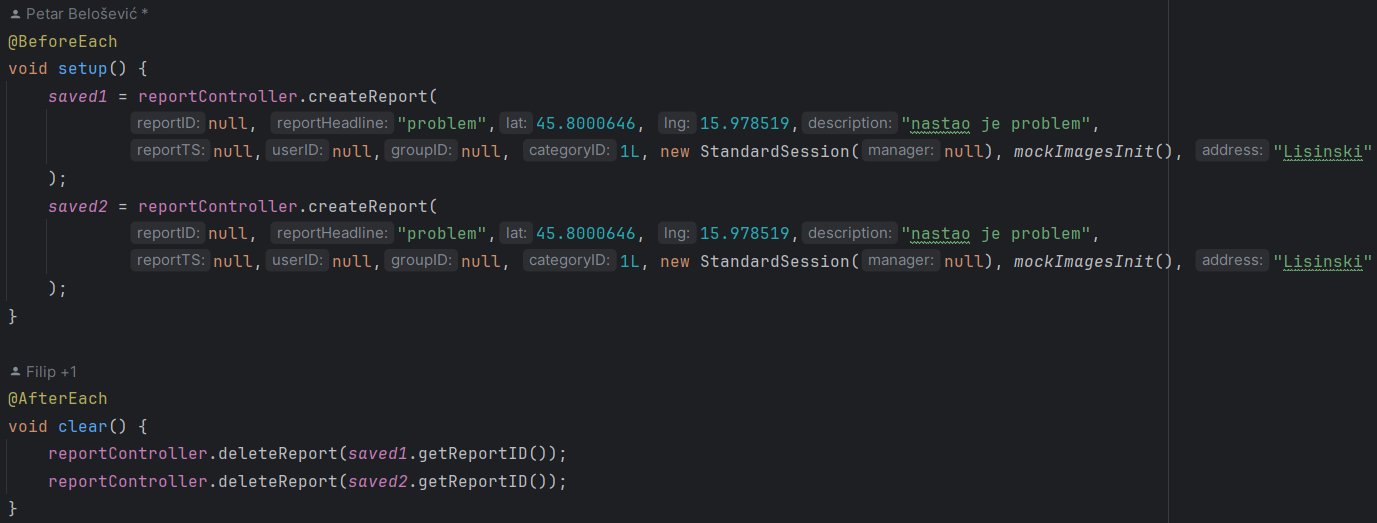
\includegraphics[width=\textwidth]{slike/JUnitTestoviPomocneMetode.png} %veličina u odnosu na širinu linije
				\caption{Pomocne metode u testovima komponenti}
				\label{fig:JUnitTestoviPomocne} %label mora biti drugaciji za svaku sliku
			\end{figure}
			
			\textbf{Test 1:}
			
			U ovom testu se prvo provjerava ako se prilikom stvaranja nove prijave njezin status automatski postavlja na "neobraden". Zatim se provjerava ako se status prijave ispravno mijenja u "uProcesu".
			
			\begin{figure}[H]
				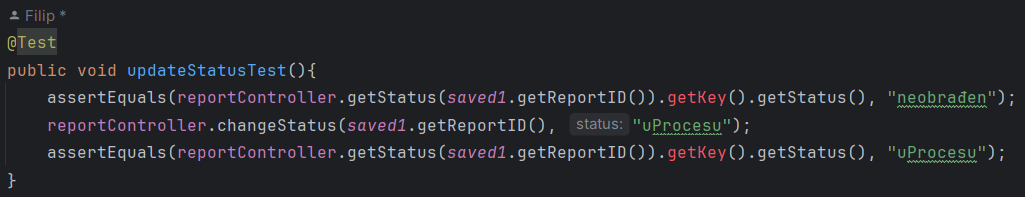
\includegraphics[width=\textwidth]{slike/JUnitTest1.png} %veličina u odnosu na širinu linije
				\caption{Test komponenti 1}
				\label{fig:JUnitTest1} %label mora biti drugaciji za svaku sliku
			\end{figure}
			
			\textbf{Test 2:}
			
			U ovom testu se provjerava ako komponenta ispravno reagira kada se više puta pokušava promijeniti status prijave na isti status. U tom slučaju pripadajuća metoda treba baciti odgovarajuću iznimku.
			
			\begin{figure}[H]
				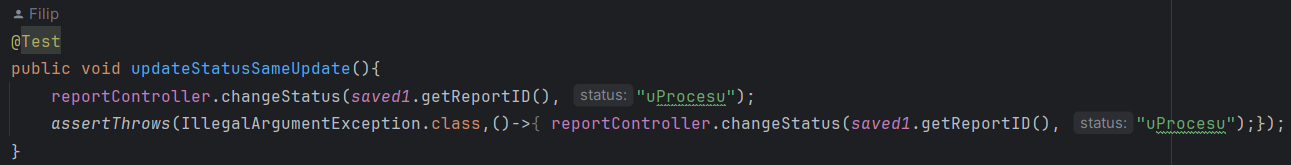
\includegraphics[width=\textwidth]{slike/JUnitTest2.png} %veličina u odnosu na širinu linije
				\caption{Test komponenti 2}
				\label{fig:JUnitTest2} %label mora biti drugaciji za svaku sliku
			\end{figure}
			
			\textbf{Test 3:}
			
			U ovom testu se ispitiva reagiranje komponente na pokušaj promjene statusa nepostojećoj prijavi, to jest prijavi sa nepostojećim ID-om. Od pripadne metode se u tom slučaju očekuje bacanje iznimke.
			
			\begin{figure}[H]
				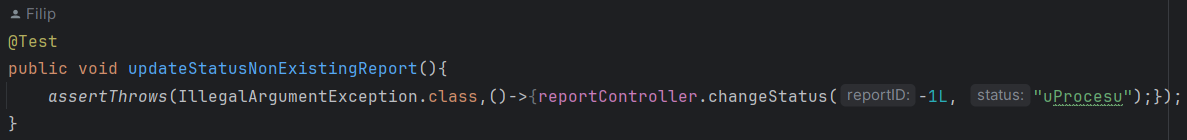
\includegraphics[width=\textwidth]{slike/JUnitTest3.png} %veličina u odnosu na širinu linije
				\caption{Test komponenti 3}
				\label{fig:JUnitTest3} %label mora biti drugaciji za svaku sliku
			\end{figure}
				
			\textbf{Test 4:}
			
			U ovom testu se ispitiva reagiranje komponente na pokušaj promjene statusa prijavi bez davanja ID-a prijave. Metodi se dakle kao ID prijave predaje null referenca. Metoda u tom slučaju treba baciti iznimku.
			
			\begin{figure}[H]
				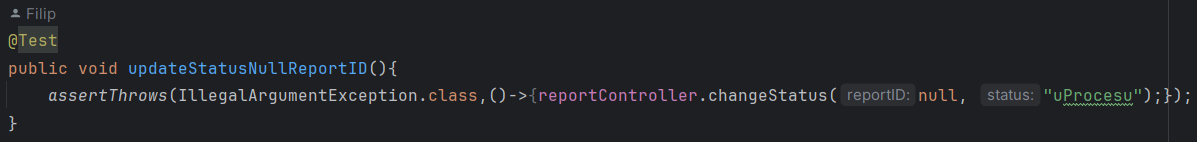
\includegraphics[width=\textwidth]{slike/JUnitTest4.png} %veličina u odnosu na širinu linije
				\caption{Test komponenti 4}
				\label{fig:JUnitTest4} %label mora biti drugaciji za svaku sliku
			\end{figure}
			
			\textbf{Test 5:}
			
			U ovom testu se prvo provjerava ako inicijalno prijava nije nadovezana niti na jednu prijavu. Zatim se druga prijava nadovezuje na prvu prijavu predajom ID-eva prijava u metodu za nadovezivanje. na kraju se provjerava ispravnost provedenog nadovezivanja.
			
			\begin{figure}[H]
				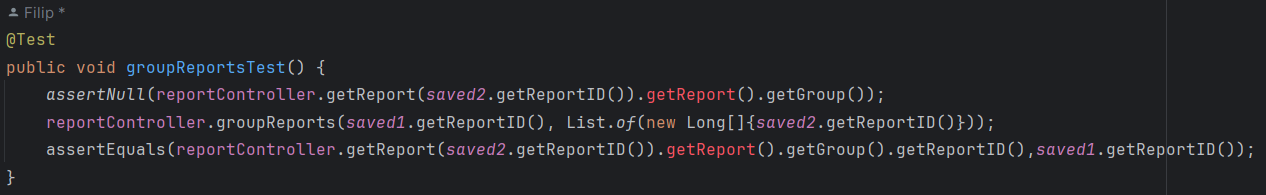
\includegraphics[width=\textwidth]{slike/JUnitTest5.png} %veličina u odnosu na širinu linije
				\caption{Test komponenti 5}
				\label{fig:JUnitTest5} %label mora biti drugaciji za svaku sliku
			\end{figure}
			
			\textbf{Test 6:}
			
			U ovom testu se provjerava ispravno ponašanje prilikom pokušaja nadovezivanja prijave uz davanje nevažećeg ID-a prijave na koju se nadovezuje. U tom slučaju pripadna metoda treba baciti iznimku.
			
			\begin{figure}[H]
				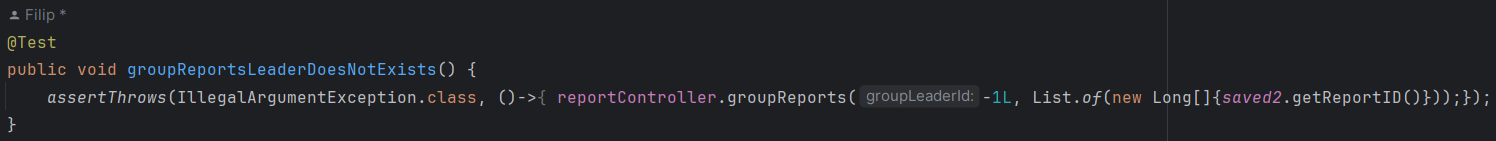
\includegraphics[width=\textwidth]{slike/JUnitTest6.png} %veličina u odnosu na širinu linije
				\caption{Test komponenti 6}
				\label{fig:JUnitTest6} %label mora biti drugaciji za svaku sliku
			\end{figure}
			
			\textbf{Test 7:}
			
			U ovom testu se provjerava ispravno ponašanje prilikom pokušaja nadovezivanja prijave bez davanja prijave na koju se nadovezuje. U tom slučaju pripadna metoda treba baciti iznimku.
			
			\begin{figure}[H]
				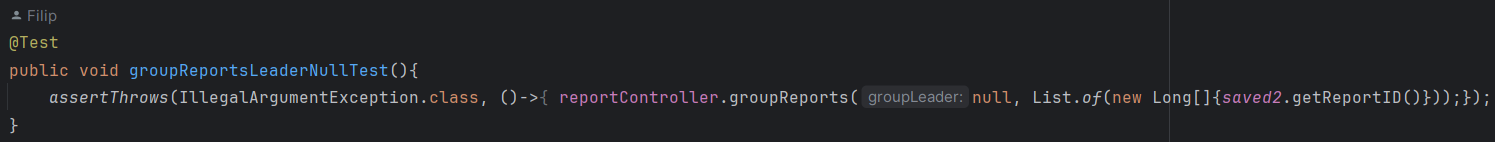
\includegraphics[width=\textwidth]{slike/JUnitTest7.png} %veličina u odnosu na širinu linije
				\caption{Test komponenti 7}
				\label{fig:JUnitTest7} %label mora biti drugaciji za svaku sliku
			\end{figure}
			
			\textbf{Test 8:}
			
			U ovom testu se provjerava ispravno ponašanje prilikom pokušaja nadovezivanja prijava bez davanja prijava koje se nadovezuju. Konkretnije, umjesto prijava koje se trebaju nadovezati predaje se null referenca. U tom slučaju pripadna metoda treba baciti iznimku.
			
			\begin{figure}[H]
				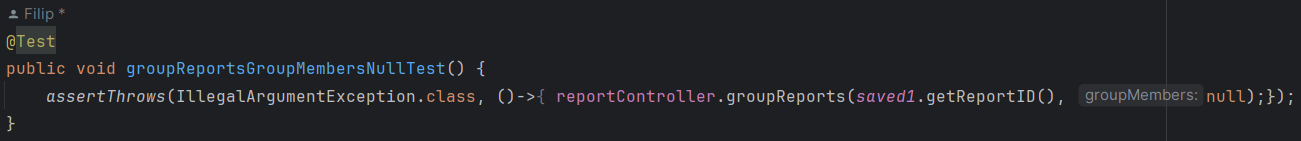
\includegraphics[width=\textwidth]{slike/JUnitTest8.png} %veličina u odnosu na širinu linije
				\caption{Test komponenti 8}
				\label{fig:JUnitTest8} %label mora biti drugaciji za svaku sliku
			\end{figure}
			
			\textbf{Test 9:}
			
			U ovom testu se provjerava ispravno ponašanje prilikom pokušaja nadovezivanja prijava uz davanje praznog polja prijava koje se nadovezuju. U tom slučaju pripadna metoda treba baciti iznimku.
			
			\begin{figure}[H]
				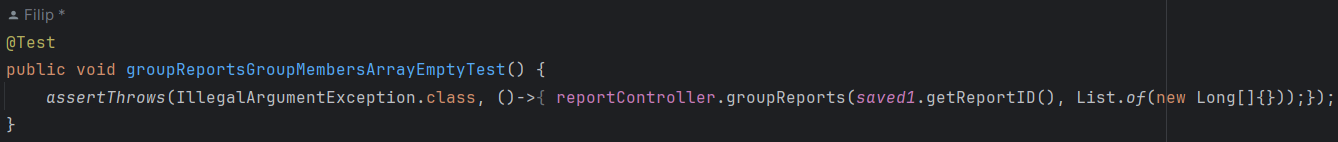
\includegraphics[width=\textwidth]{slike/JUnitTest9.png} %veličina u odnosu na širinu linije
				\caption{Test komponenti 9}
				\label{fig:JUnitTest9} %label mora biti drugaciji za svaku sliku
			\end{figure}
			
			\textbf{Test 10:}
			
			U ovom testu se pokušava napraviti nadovezivanje prijave na samu sebe. Takva radnja očekuje izazivanje iznimke.
			
			\begin{figure}[H]
				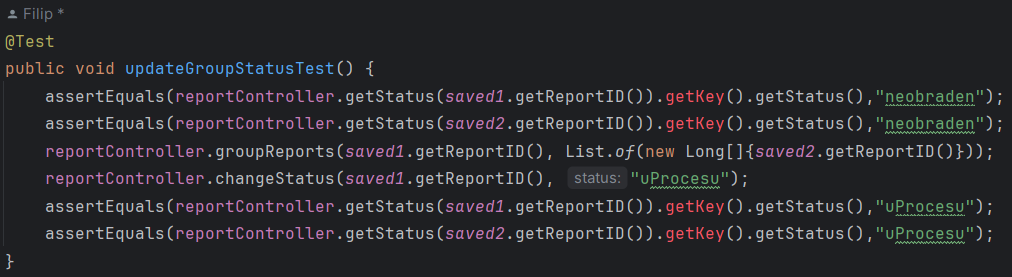
\includegraphics[width=\textwidth]{slike/JUnitTest10.png} %veličina u odnosu na širinu linije
				\caption{Test komponenti 10}
				\label{fig:JUnitTest10} %label mora biti drugaciji za svaku sliku
			\end{figure}
			
			\textbf{Test 11:}
			
			U ovom testu se provjerava ispravnost promjene statusa povezanih prijava. Prvo se provjerava ako prijave imaju status "neobraden". Zatim se druga prijava nadovezuje na prvu te se prvoj prijavi mijenja status u "uProcesu". Očekuje se da promjena nad glavnom prijavom rezultira istom promjenom i u svim nadovezanim prijavama. Stoga se na kraju provjerava ako obje prijave imaju promjenjen status u "uProcesu".
			
			\begin{figure}[H]
				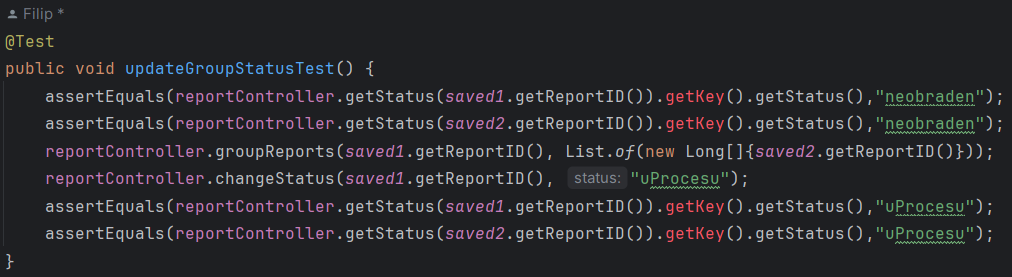
\includegraphics[width=\textwidth]{slike/JUnitTest11.png} %veličina u odnosu na širinu linije
				\caption{Test komponenti 11}
				\label{fig:JUnitTest11} %label mora biti drugaciji za svaku sliku
			\end{figure}
			
			
			\subsection{Ispitivanje sustava}
		 	
		 	Ispitivanje sustava kao cjeline odrađeno je pomoću Selenium WebDrivera za Chrome koji se koristio unutar JUnit testova. Svi testovi su uspješno prošli.
		 	
		 	\begin{figure}[H]
		 		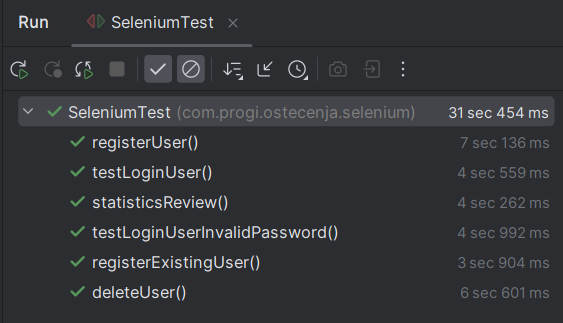
\includegraphics[width=\textwidth]{slike/SeleniumTestoviRez.png} %veličina u odnosu na širinu linije
		 		\caption{Rezultati ispitivanja sustava}
		 		\label{fig:SeleniumTestovi} %label mora biti drugaciji za svaku sliku
		 	\end{figure}
		 	
		 	Prije svakog testa se inicijalizira ChromeDriver u posebnoj metodi te se na kraju svakog testa inicijalizirani ChromeDriver gasi u posebnoj metodi.
		 	
		 	\begin{figure}[H]
		 		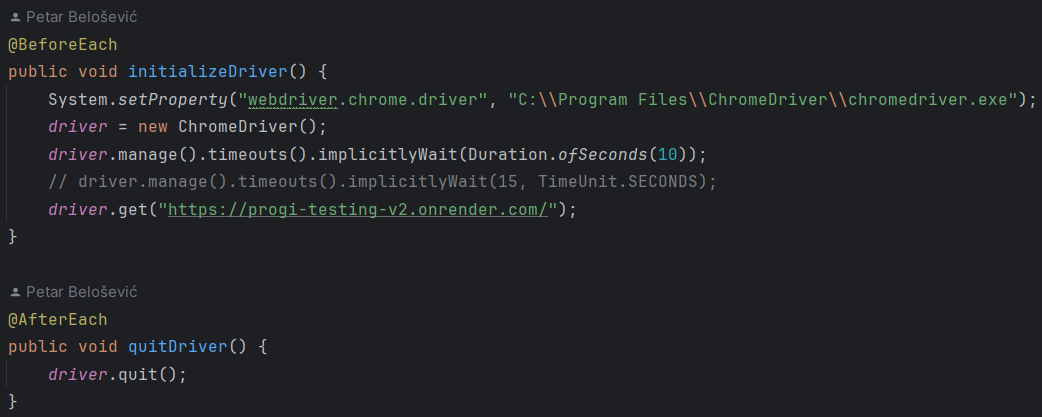
\includegraphics[width=\textwidth]{slike/SeleniumTestoviPomocneMetode.png} %veličina u odnosu na širinu linije
		 		\caption{Pomočne metode za ispitivanje sustava}
		 		\label{fig:SeleniumTestoviPomocneMetode} %label mora biti drugaciji za svaku sliku
		 	\end{figure}
		 	
		 	\textbf{Test 1:}
		 	
		 	U ovom testu se ispituje rad sustava tijekom pokušaja prijave korisnika koji postoji u bazi podataka. Simulira se odabir opcije prijave korisnika na korisničkom sučelju. U obrazac za prijavu se upisuju podaci "abc@gmail.com" za e-mail i "pass1234" za lozinku te se klikne na gumb za prijavu. Očekuje se da prijava bude uspješna. To treba rezultirati preusmjeravanjem na glavnu stranicu te prikazom gumba sa korisnikovom e-mail adresom u zaglavlju stranice.
		 	
		 	\begin{figure}[H]
		 		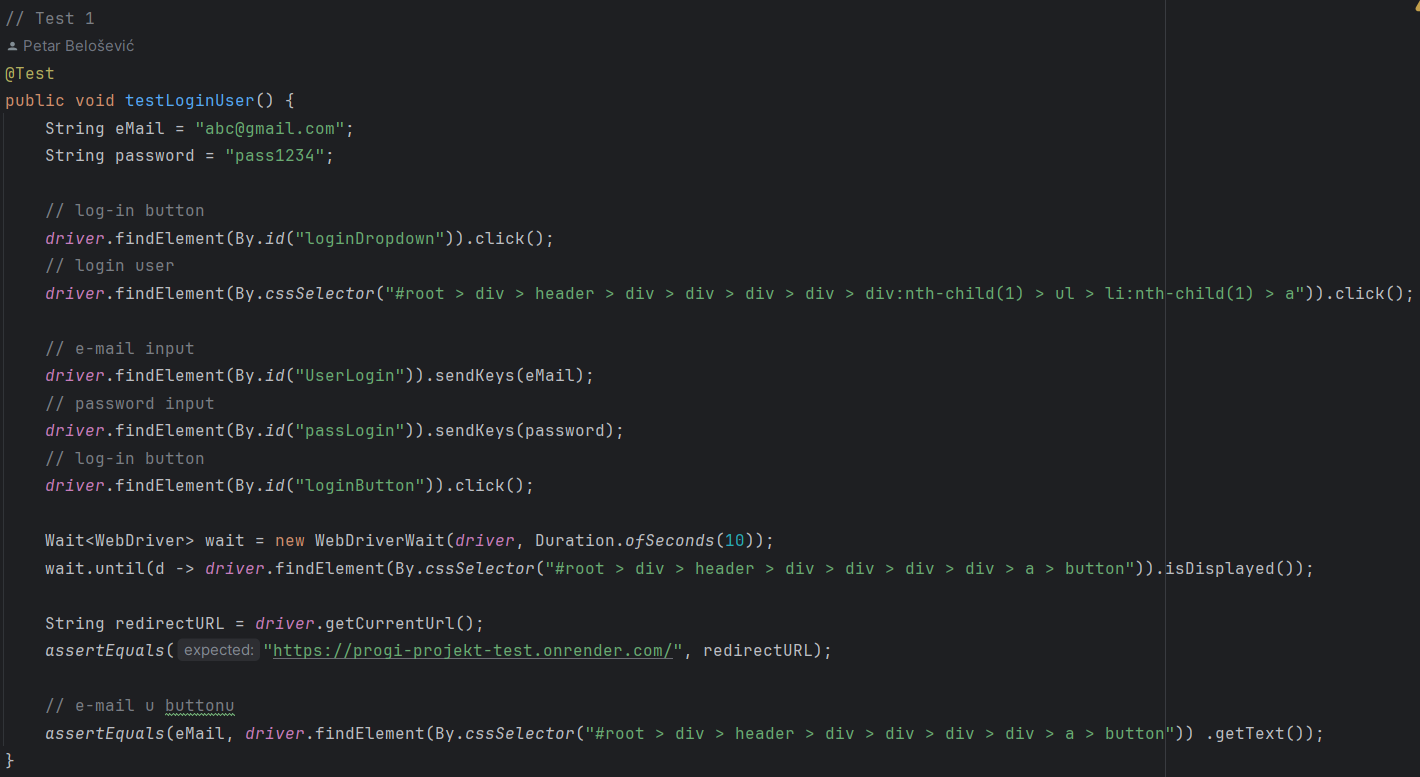
\includegraphics[width=\textwidth]{slike/SeleniumTest1.png} %veličina u odnosu na širinu linije
		 		\caption{Ispitivanje sustava: Test 1}
		 		\label{fig:SeleniumTest1} %label mora biti drugaciji za svaku sliku
		 	\end{figure}
		 	
		 	\textbf{Test 2:}
		 	
		 	Ovaj test je ispitivanje pokušaja prijave korisnika s neispravnom lozinkom. Radnje ovog testa su iste kao i u prethodnom testu. Razlika je što se na kraju ne očekuje preusmjeravanje na glavnu stranicu već prikaz prozora sa porukom "Greška kod prijave: neispravan mail ili lozinka!".
		 	
		 	\begin{figure}[H]
		 		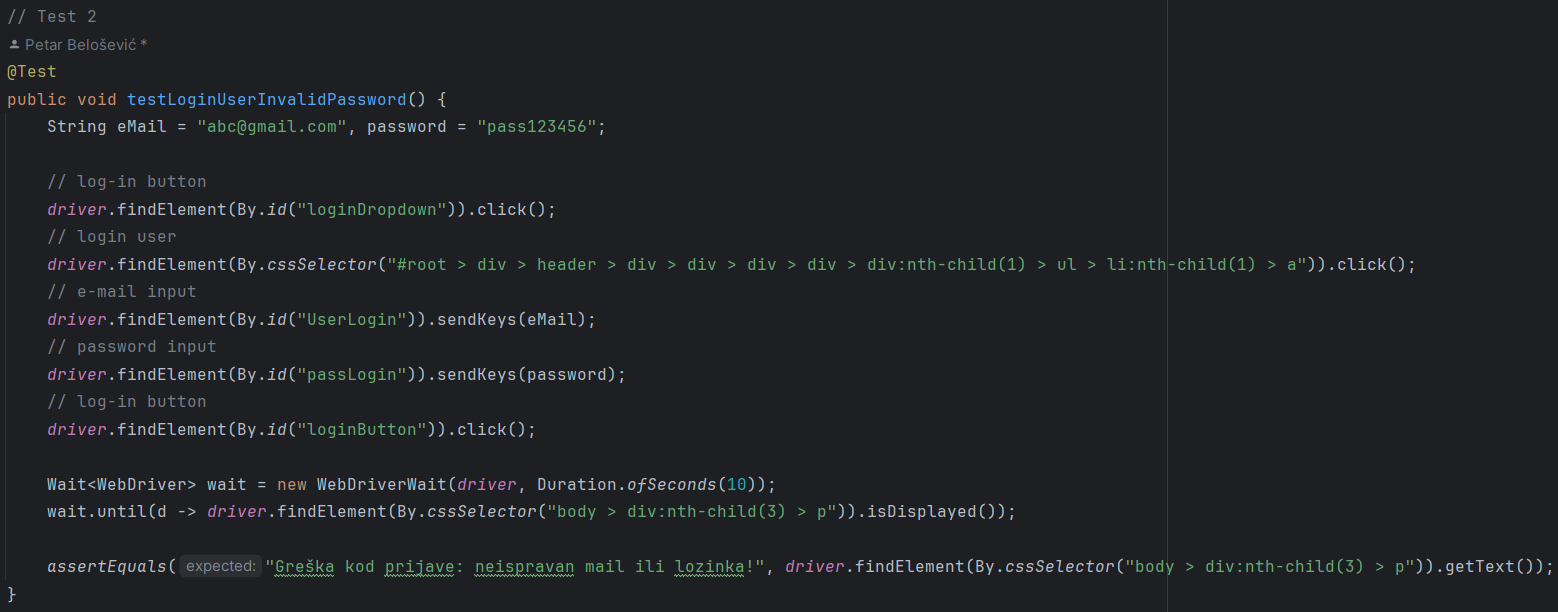
\includegraphics[width=\textwidth]{slike/SeleniumTest2.png} %veličina u odnosu na širinu linije
		 		\caption{Ispitivanje sustava: Test 2}
		 		\label{fig:SeleniumTest2} %label mora biti drugaciji za svaku sliku
		 	\end{figure}
		 	
		 	\textbf{Test 3:}
		 	
		 	U ovom se testu ispituje pokušaj registracije novog korisnika. Simulira se odabir opcije registracije novog korisnika. Na novoj se stranici u obrazac upisuju podaci "Ime" za ime, "Prezime" za prezime, "novi.user.1@gmail.com" za e-mail i "lozinka123" za lozinku. Na kraju se registracija dovršava pritiskom gumba za registraciju. Očekuje se uspješna registracija što rezultira preusmjeravanjem na početnu stranicu te prikazom gumba sa korisnikovom e-mail adresom u zaglavlju stranice.
		 	
		 	\begin{figure}[H]
		 		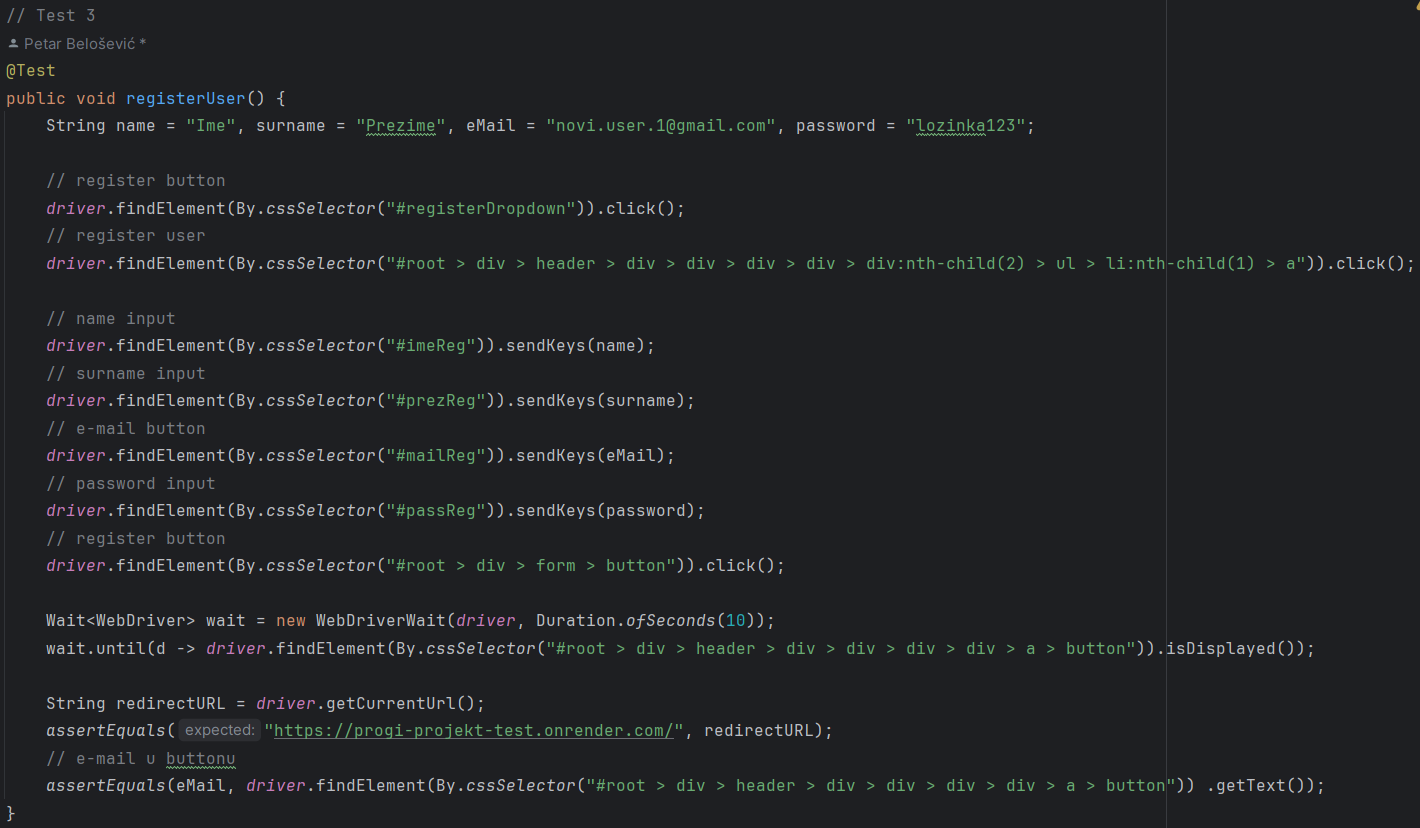
\includegraphics[width=\textwidth]{slike/SeleniumTest3.png} %veličina u odnosu na širinu linije
		 		\caption{Ispitivanje sustava: Test 3}
		 		\label{fig:SeleniumTest3} %label mora biti drugaciji za svaku sliku
		 	\end{figure}
		 	
		 	\textbf{Test 4:}
		 	
		 	U ovom testu se ispituje sustav prilikom pokušaja registracije korisnika koji već postoji u sustavu, to jest sa već iskorištenom e-mail adresom. Ponavljaju se radnje iz prošlog testa, ali se u obrazac za registraciju unose drugi podaci. Za ovaj test se unose podaci "xx" za ime, "yy" za prezime, "abc@gmail.com" za e-mail i "pass1234" za lozinku. S obzirom da korisnik s danom e-mail adresom već postoji u sustavu. Aplikacija treba prikazati pripadnu poruku te nakon klika na gumb uz poruku treba ostati na stranici za registraciju.
		 	
		 	\begin{figure}[H]
		 		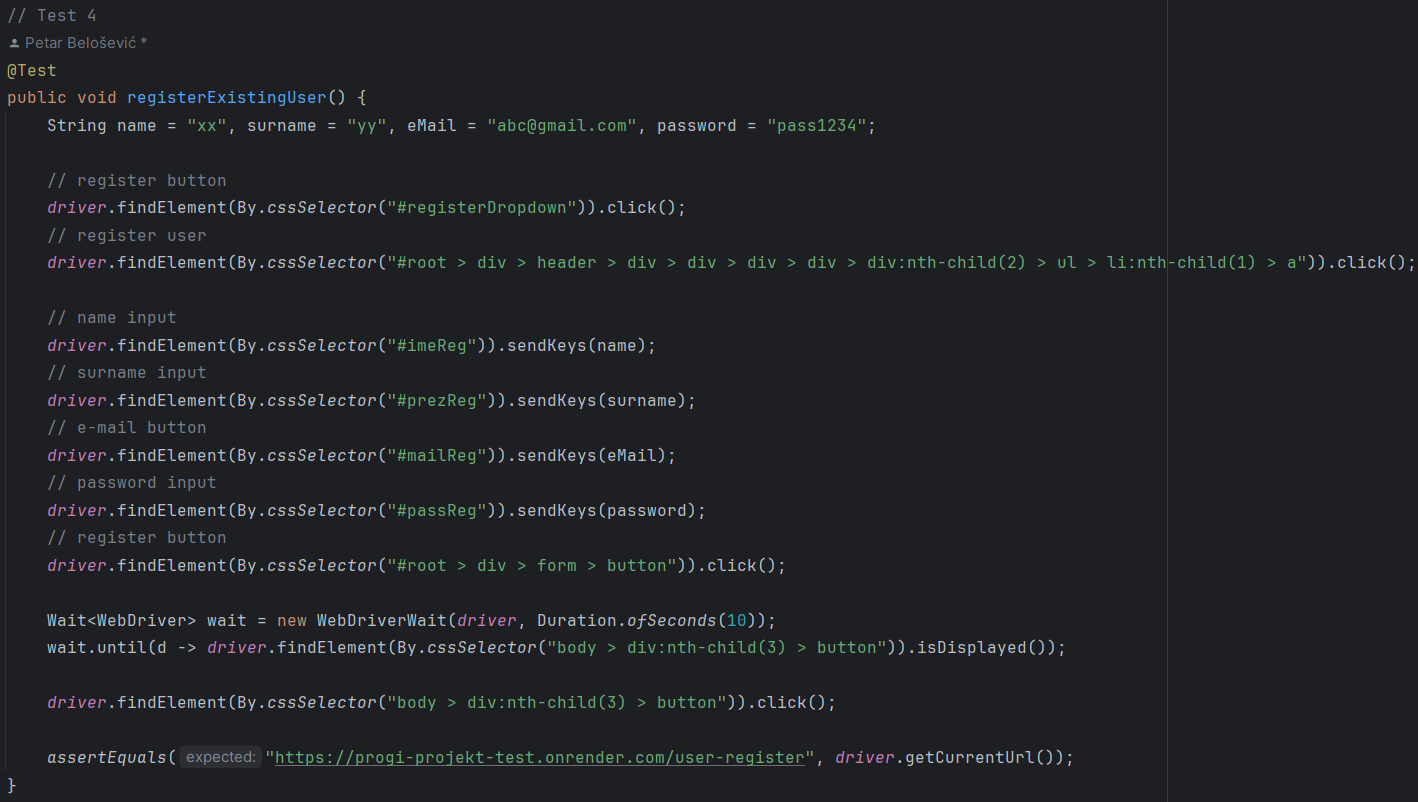
\includegraphics[width=\textwidth]{slike/SeleniumTest4.png} %veličina u odnosu na širinu linije
		 		\caption{Ispitivanje sustava: Test 4}
		 		\label{fig:SeleniumTest4} %label mora biti drugaciji za svaku sliku
		 	\end{figure}
		 	
		 	\textbf{Test 5:}
		 	
		 	U ovom testu se pokušava izbrisati korisnika iz sustava. Simulira se prijava korisnika u sustav sa podacima "novi.user.1@gmail.com" za e-mail i "lozinka123" (korisnik koji se registrirao u ranijem testu) kao što je opisano u testu 1. Zatim se klikom na gumb sa korisnikovim e-mailom i odabirom profilne stranice odlazi na stranicu korisnikovog profila. Tamo se simulira klik na gumb za brisanje računa nakon čega se prikazuje prozor sa porukom "Profile successfully deleted" i pripadnim gumbom. Pritiskom na gumb se korisnika treba preusmjeriti na glavnu stranicu.
		 	
		 	\begin{figure}[H]
		 		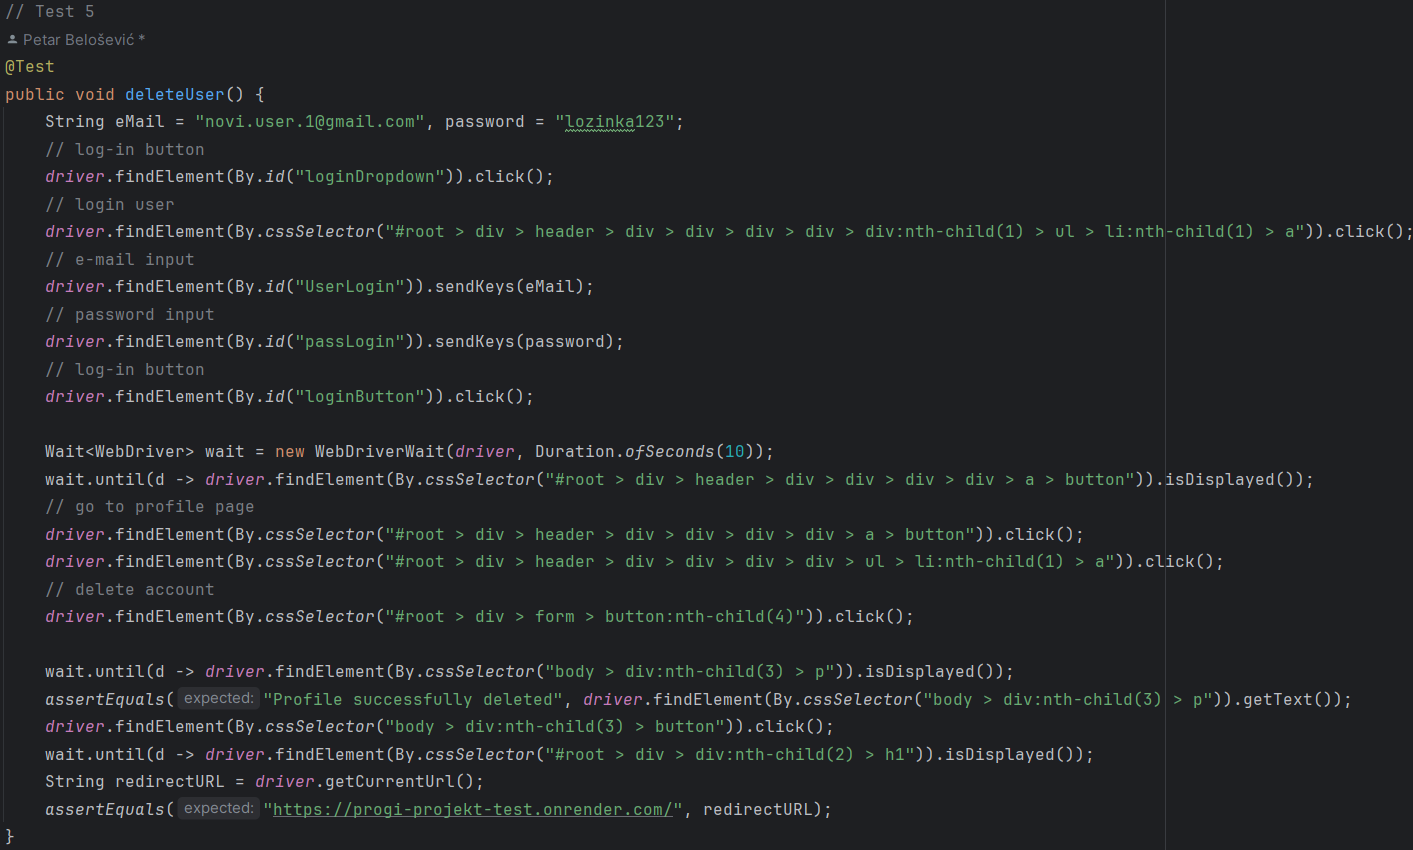
\includegraphics[width=\textwidth]{slike/SeleniumTest5.png} %veličina u odnosu na širinu linije
		 		\caption{Ispitivanje sustava: Test 5}
		 		\label{fig:SeleniumTest5} %label mora biti drugaciji za svaku sliku
		 	\end{figure}
		 	
		 	\textbf{Test 6:}
		 	
		 	U ovom testu se simulira pregledavanje statistike prijava. Klikom na gumb "Statistika" u zaglavlju stranice korisnika se preusmjerava na stranicu za statistiku.  Na prikazanoj stranici se djelomično popunjava obrazac za prikaz statistike. Za kategoriju se odabire prva kategorija koja počinje na "r", za datum početka se odabire 1.1.2024., a za datum završetka intervala se odabire 2.2.2024. Tako popunjen obrazac se šalje na poslužitelja. Nakon toga se ispod filtra očekuje prikaz statističkih podataka o prijavama odabranima poslanim filtrom.
		 	
		 	\begin{figure}[H]
		 		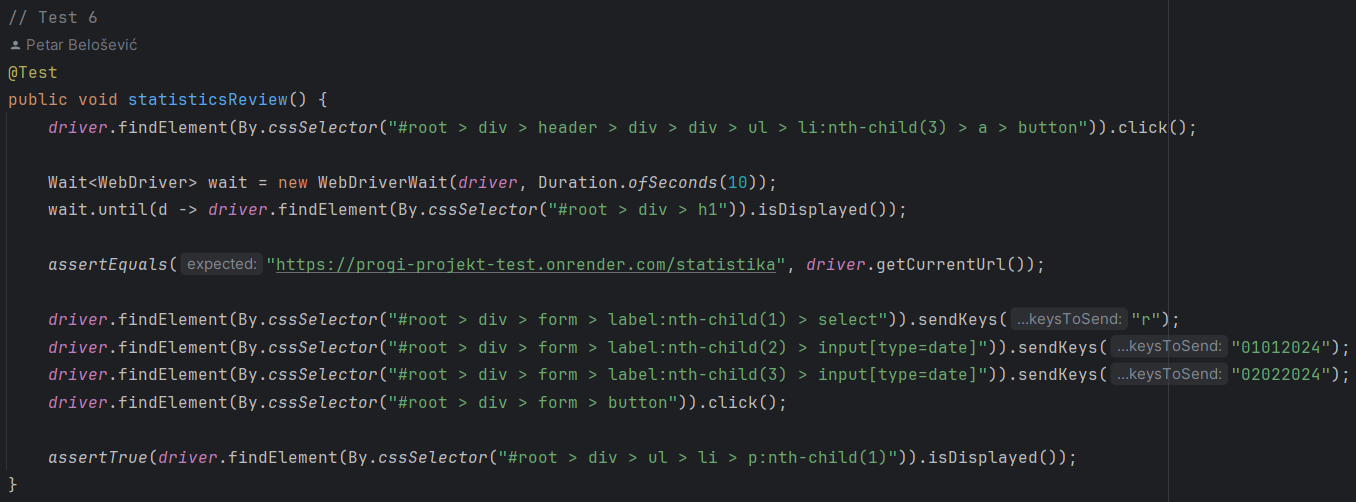
\includegraphics[width=\textwidth]{slike/SeleniumTest6.png} %veličina u odnosu na širinu linije
		 		\caption{Ispitivanje sustava: Test 6}
		 		\label{fig:SeleniumTest6} %label mora biti drugaciji za svaku sliku
		 	\end{figure}
			
			\eject 
		
		
		\section{Dijagram razmještaja}
			
			\textbf{\textit{dio 2. revizije}}
			
			Dijagram razmještaja je statički strukturni dijagram koji opisuje topologiju sutava i usredotočen je na odnos sklopovskih i programskih dijelova. Osnovni elementi dijagrama su čvorovi, artefakti i spojevi.
			
			Dijagram \ref{fig:dijagramRazmjestaja} prikazuje topologiju sustava za prijavljivanje oštećenja na javnim površinama. Sustav je napravljen na temelju arhitekture klijent-poslužitelj u kojoj klijent i poslužitelj komuniciraju HTTPS protokolom. Sustav je stavljen u pogon pomoću dva odvojena servisa na usluzi Render, jedan za aplikaciju i jedan za bazu podataka. Na Render servisu za bazu podataka postoji instanca PostgreSQL baze podataka te taj servis prima zahtjeve za bazu podataka na standardnom portu 5432. Na Render servisu za web aplikaciju je pokrenut Docker kontejner unutar kojeg su upogonjeni React frontend i Spring Boot backend dijelovi aplikacije. Spring Boot backend po potrebi komunicira sa bazom podataka slanjem SQL querryja na port 5432 Render servisa za bazu podataka. Render servis za web aplikaciju sluša HTTPS zahtjeve na portu 443. Zaprimljene HTTPS zahtjeve Render servis prosljeđuje na port 8080 Docker kontejnera kao HTTP zahtjeve. Klijentski uređaj na sebi ima pokrenuti web preglednik pomoću kojeg šalje HTTPS zahtjeve na port 443 Render servisa za web aplikaciju.
			
			\begin{figure}[H]
				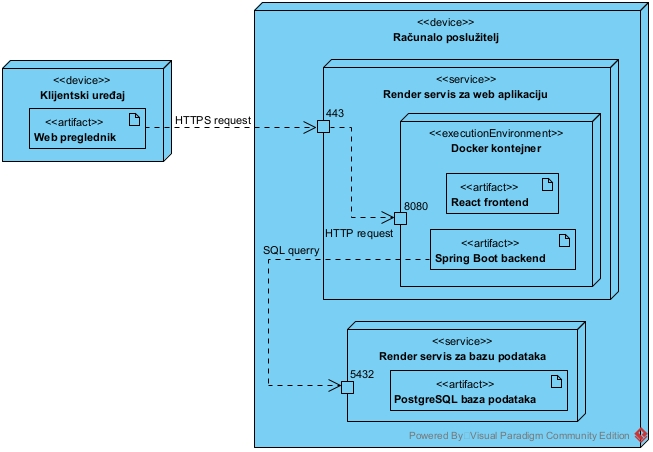
\includegraphics[width=\textwidth]{slike/dijagramRazmjestaja.jpg} %veličina u odnosu na širinu linije
				\caption{Dijagram razmještaja}
				\label{fig:dijagramRazmjestaja} %label mora biti drugaciji za svaku sliku
			\end{figure}
			
			\eject 
		
		\section{Upute za puštanje u pogon}
		
			\textbf{\textit{dio 2. revizije}}\\
			
			Ovaj sustav je pušten u pogon pomoću online servisa Render pa se u uputama za puštanje u pogon pretpostavlja korištenje istog. Za tu svrhu potrebno je napraviti korisnički račun na Renderu. 
			
			\subsection{Konfiguracija poslužitelja baze podataka}
			
			Potrebno je odabrati opciju stvaranja nove PostgreSQL baze podataka.
			
			\begin{figure}[H]
				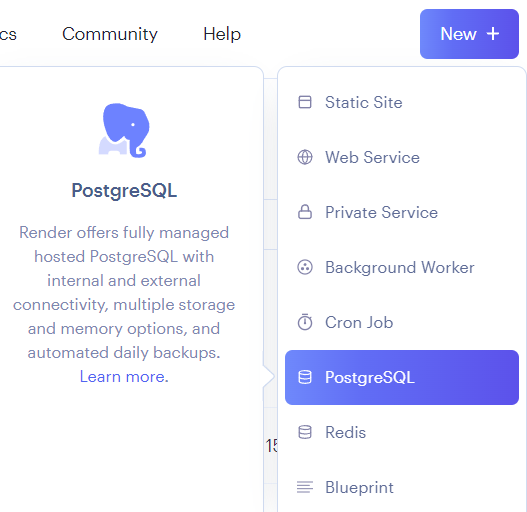
\includegraphics[scale=0.8]{slike/upute/odabirStvaranjaBaze.png} %veličina u odnosu na širinu linije
				\centering
				\caption{Odabir stvaranja nove baze podataka}
				\label{fig:odabirStvaranjaBaze} %label mora biti drugaciji za svaku sliku
			\end{figure}
			
			Zatim je potrebno konfigurirati bazu.
			
			\begin{figure}[H]
				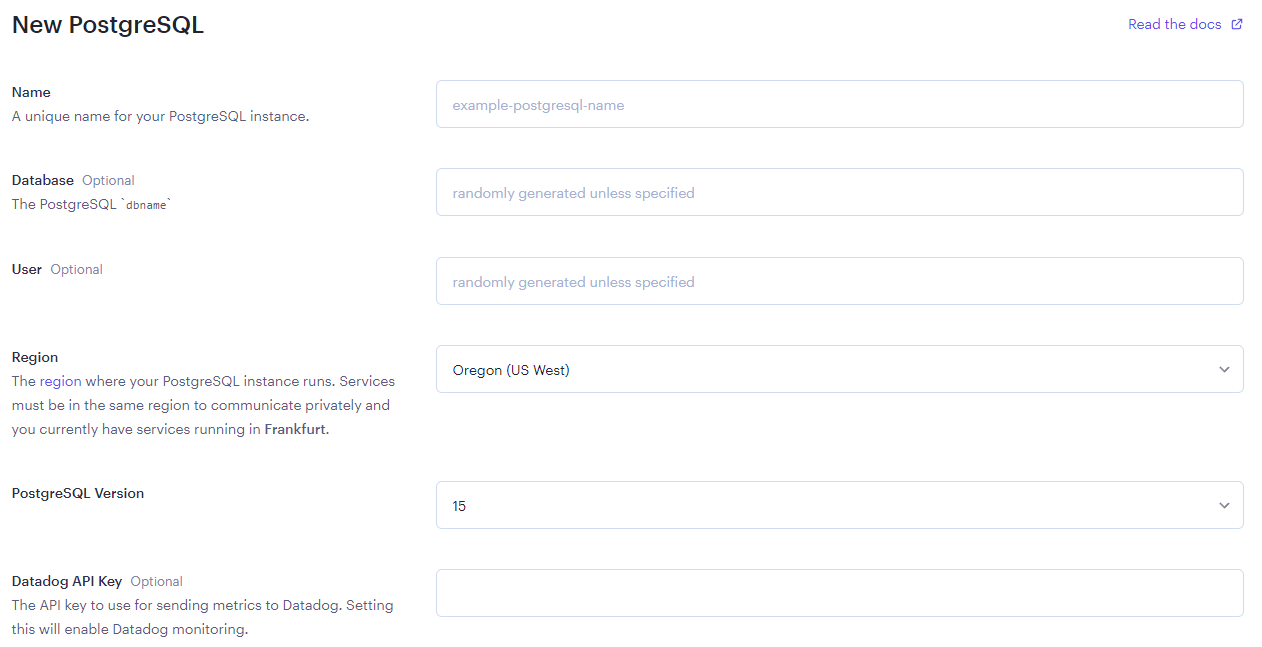
\includegraphics[width=\textwidth]{slike/upute/konfiguriranjeBaze.png} %veličina u odnosu na širinu linije
				\caption{Konfiguriranje baze podataka}
				\label{fig:konfiguriranjeBaze} %label mora biti drugaciji za svaku sliku
			\end{figure}
			
			Za ime instance baze podataka, ime same baze i ime korisnika se mogu unesti proizvoljna imena. Za regiju je poželjno odabrati geografski najbližu regiju, s obzirom da će to rezultirati najmanjom latencijom. U našem slučaju najbliža regija bila je \textit{Frankfurt (EU Central)}. Ostale parametre nije potrebno mijenjati.
			
			\begin{figure}[H]
				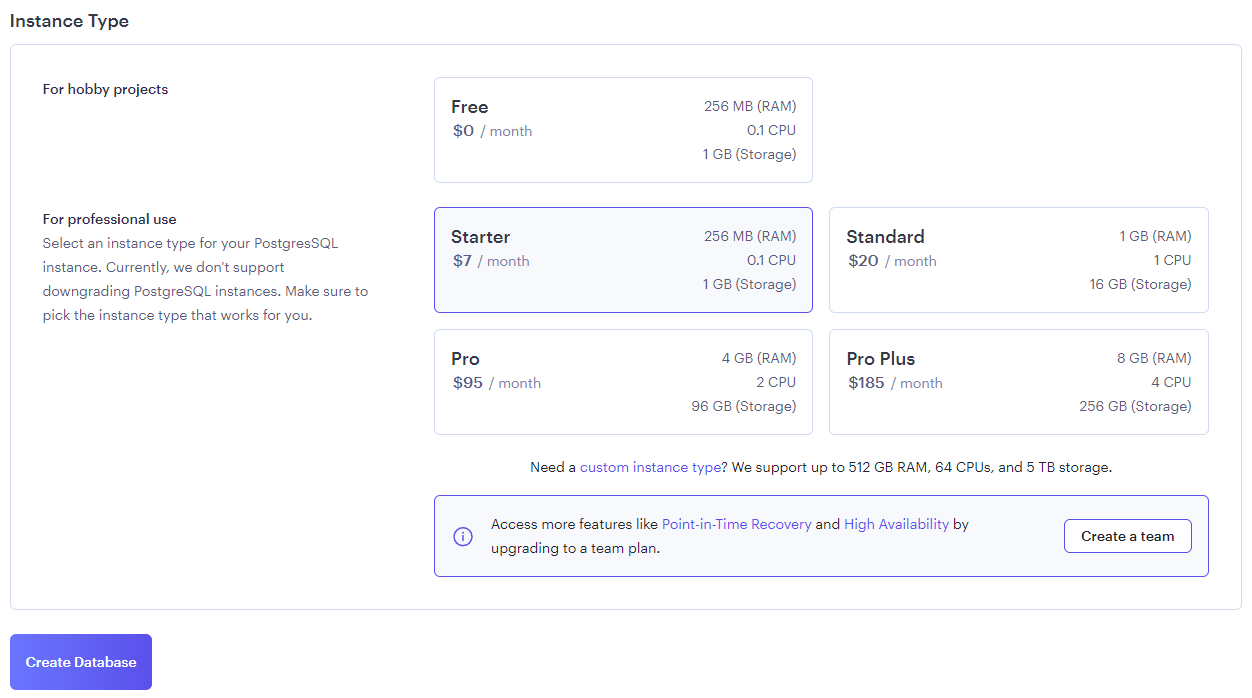
\includegraphics[width=\textwidth]{slike/upute/bazaPlacanje.png} %veličina u odnosu na širinu linije
				\caption{Odabir vrste instance baze podataka}
				\label{fig:bazaPlacanje} %label mora biti drugaciji za svaku sliku
			\end{figure}
			
			Sljedeće je potrebno odabrati vrstu instance baze podataka, odnosno cjenovni rang baze. Ovo je isključivo pitanje preference osobe koja pušta sustav u pogon, odnosno koliko je spremna platiti za puštanje baze podataka u pogon. Za naše potrebe bilo je dovoljna besplatna opcija te smo istu i odabrali.
			
			Nakon toga treba kliknuti na \textit{Create Database} i time će baza biti puštena u pogon.
			
			\subsection{Konfiguracija poslužitelja web aplikacije}
			
			Prije puštanja aplikacije u pogon potrebno je u Git repozitoriju ažurirati podatke za spajanje s bazom podataka. Za to je potrebno izmjeniti vrijednosti varijabli \textit{spring.datasource.url}, \textit{spring.datasource.username} i \textit{spring.datasource.password} u datoteci \textit{IzvorniKod/server/src/main/resources/application.properties} u \textit{main} grani repozitorija. 
			
			\begin{figure}[H]
				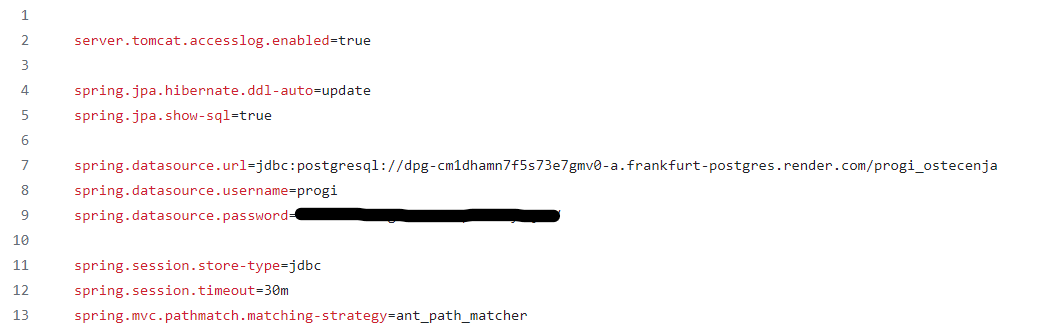
\includegraphics[width=\textwidth]{slike/upute/applicationProperties.png} %veličina u odnosu na širinu linije
				\caption{Datoteke s podacima za spajanje s bazom podataka}
				\label{fig:applicationProperties} %label mora biti drugaciji za svaku sliku
			\end{figure}
			
			Na web stranici Rendera potrebno je odabrati karticu \textit{Dashboard} i zatim odabrati ranije upogonjenu bazu podataka. Na novootvorenoj stranici potrebno je pronaći odjeljak \textit{Connections} gdje se nalaze potrebni parametri. vrijednosti \textit{Username} i \textit{Password} potrebno je kopirati u pripadajuće varijable u datoteci na Git repozitoriju. U varijabli \textit{spring.datasource.url} potrebno je zamijeniti tekst koji slijedi nakon \textit{jdbc:postgresql://}. Taj tekst potrebno je zamijeniti dijelom varijable \textit{External Database URL} na Renderu koji započinje sa "dpg-", a prethodi mu znak '@'. Dakle, vrijednost varijable \textit{spring.datasource.url} mora započeti sa "jdbc:postgresql://dpg-...".
			
			\begin{figure}[H]
				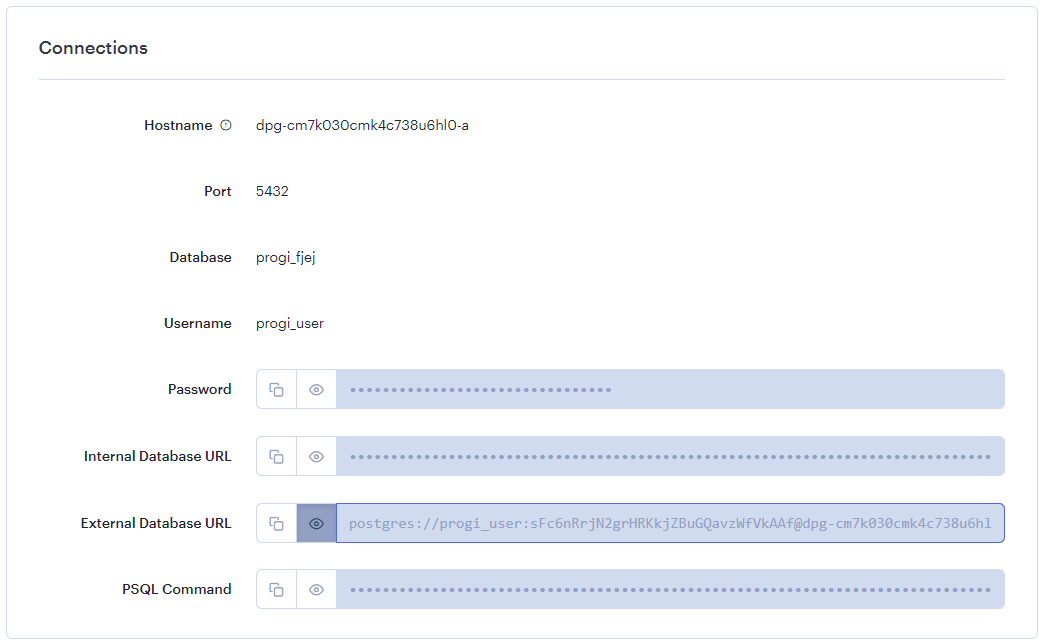
\includegraphics[width=\textwidth]{slike/upute/parametriBaze.png} %veličina u odnosu na širinu linije
				\caption{Datoteke s podacima za spajanje s bazom podataka}
				\label{fig:parametriBaze} %label mora biti drugaciji za svaku sliku
			\end{figure}
			
			Zatim je na Renderu potrebno odabrati opciju stvaranja novog web servisa.
			
			\begin{figure}[H]
				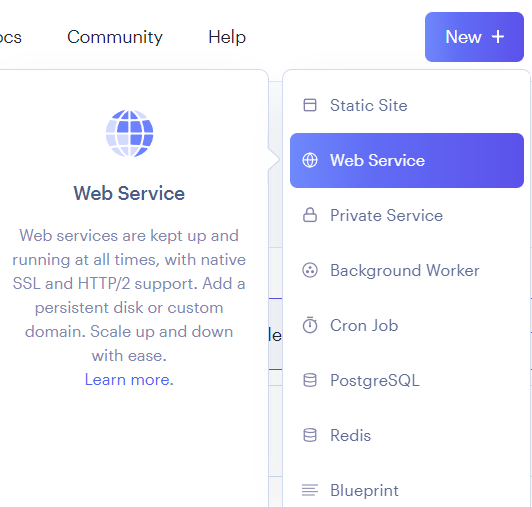
\includegraphics[scale=0.8]{slike/upute/odabirStvaranjaWebServisa.png} %veličina u odnosu na širinu linije
				\centering
				\caption{Odabir stvaranja novog web servisa}
				\label{fig:odabirStvaranjaWebServisa} %label mora biti drugaciji za svaku sliku
			\end{figure}
			
			Sljedeće je potrebno odabrati opciju izgradnje i upogonjavanja iz Git repozitorija.
			
			\begin{figure}[H]
				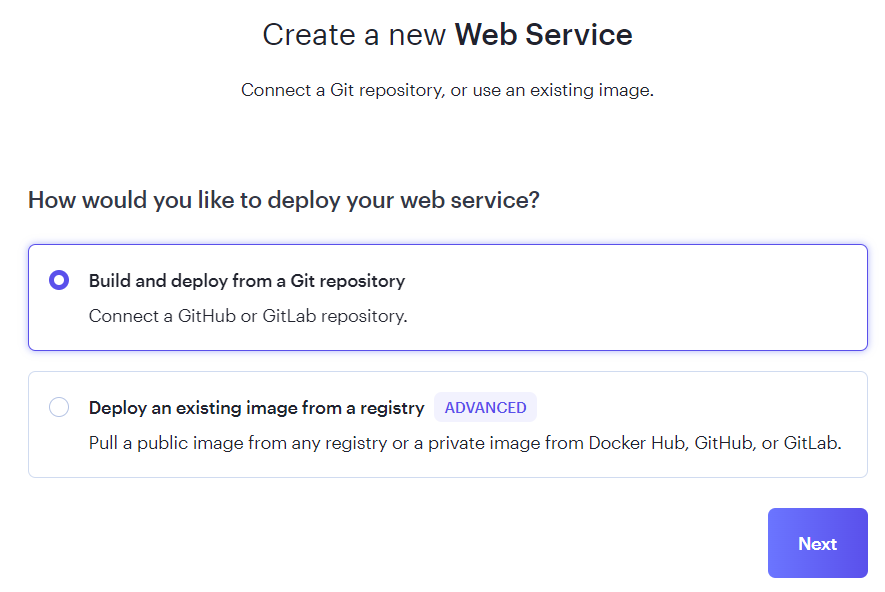
\includegraphics[width=\textwidth]{slike/upute/odabirIzvoraIzgradnje.png} %veličina u odnosu na širinu linije
				\caption{Odabir načina izgradnje}
				\label{fig:odabirIzvoraIzgradnje} %label mora biti drugaciji za svaku sliku
			\end{figure}
			
			Nakon toga potrebno je odabrati pripadni repozitorij ili unijeti URL repozitorija. Zatim slijedi konfiguracija web servisa.
			
			\begin{figure}[H]
				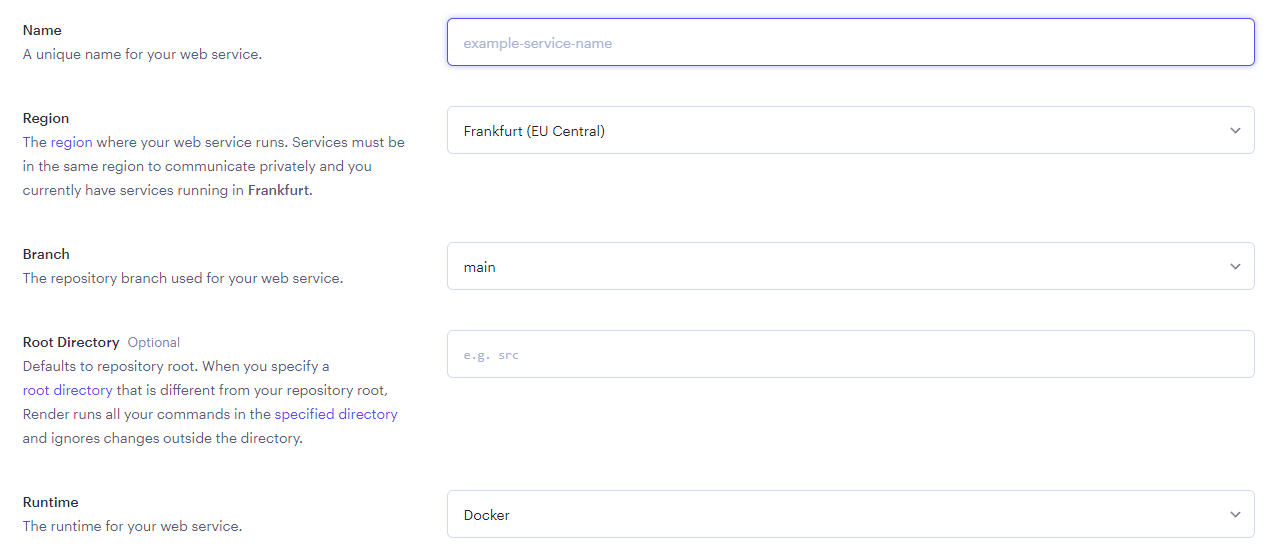
\includegraphics[width=\textwidth]{slike/upute/konfiguriranjeWebServisa.png} %veličina u odnosu na širinu linije
				\caption{Konfiguriranje web servisa}
				\label{fig:konfiguriranjeWebServisa} %label mora biti drugaciji za svaku sliku
			\end{figure}
			
			Za \textit{Name} je potrebno unesti proizvoljan naziv web servisa. Uneseno ime će biti dio URL-a samog web servisa preko kojeg će mu se moći pristupiti. Za regiju je ponovno poželjno odabrati geografski najbližu regiju što je u našem slučaju \textit{Frankfurt (EU Central)}. \textit{Branch} koji se koristi za stvaranje web servisa je potrebno ostaviti na \textit{main}. \textit{Root Directory} je potrebno ostaviti prazno. Za \textit{Runtime} je potrebno odabrati \textit{Docker}.
			
			\begin{figure}[H]
				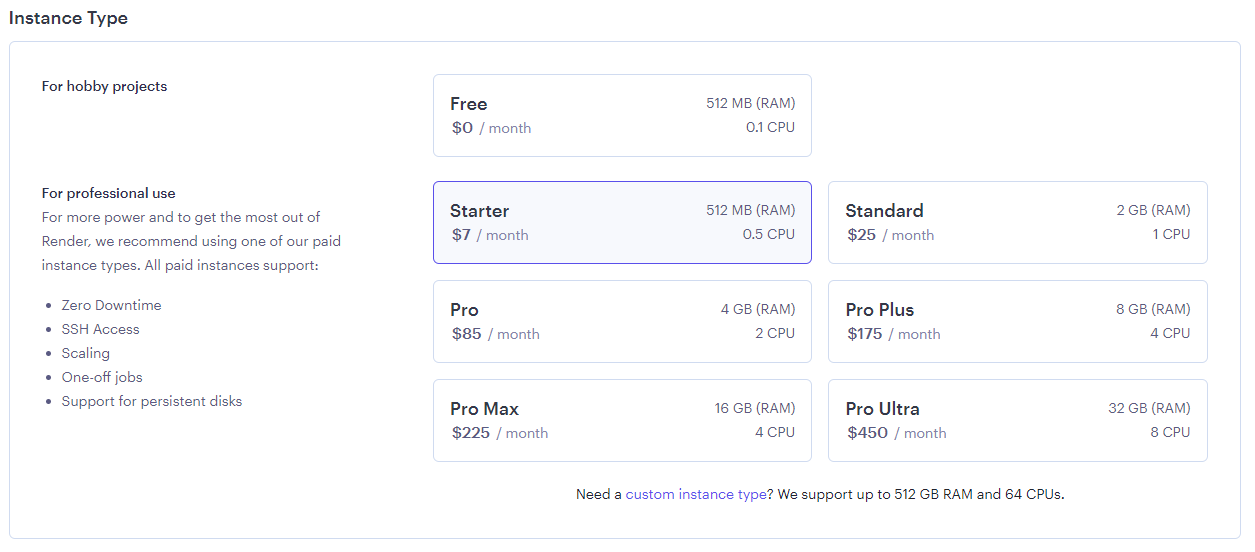
\includegraphics[width=\textwidth]{slike/upute/webServisPlacanje.png} %veličina u odnosu na širinu linije
				\caption{Odabir vrste instance web servisa}
				\label{fig:webServisPlacanje} %label mora biti drugaciji za svaku sliku
			\end{figure}
			
			Sljedeće je potrebno odabrati vrstu instance web servisa, odnosno njegov cjenovni rang. Ovo je isključivo pitanje preference osobe koja pušta sustav u pogon, odnosno koliko je spremna platiti za puštanje web serivsa u pogon. Za naše potrebe bilo je dovoljna besplatna opcija te smo istu i odabrali.
			
			Nakon treba kliknuti na \textit{Create Web Service} i time će web servis biti puštena u pogon. Prilikom prvog pokretanja web servisa baza podataka će se napuniti inicijalnim podacima.
			
			U bazi će biti sljedeći podaci:
			\begin{packed_item}
				\item Korisnici:
				\begin{packed_item}
					\item e-mail: abc@gmail.com, ime: xx, prezime: yy, lozinka: pass1234
					\item e-mail: abc2@gmail.com, ime: xx, prezime: yy, lozinka: pass1234
					\item e-mail: abc3@gmail.com, ime: xx, prezime: yy, lozinka: pass1234
					\item e-mail: abc4@gmail.com, ime: xx, prezime: yy, lozinka: pass1234
				\end{packed_item}
				\item Gradski uredi:
				\begin{packed_item}
					\item ime: Rupasti, e-mail: rupasti@gmail.com, lozinka: password
					\item ime: Rasvjeta, e-mail: rasvjeta@gmail.com, lozinka: password
					\item ime: Smece, e-mail: smece@gmail.com, lozinka: password
					\item ime: Korupcija, e-mail: korupcija@gmail.com, lozinka: password
				\end{packed_item}
				\item Kategorije:
				\begin{packed_item}
					\item kategorija: rupa na cesti, ured: Rupasti
					\item kategorija: rupa na pjesackome, ured: Rupasti
					\item kategorija: ulicna rasvjeta, ured: Rasvjeta
					\item kategorija: smece na ulici, ured: Smece
					\item kategorija: smece u parku, ured: Smece
					\item kategorija: institucionalna korupcija, ured: Korupcija
				\end{packed_item}
				\item Ključne riječi za kategorije:
				\begin{packed_item}
					\item riječ: Rupa, kategorija: rupa na cesti
					\item riječ: Cesta, kategorija: rupa na cesti
					\item riječ: Pjesacki, kategorija: rupa na pjesackome
					\item riječ: Pješački, kategorija: rupa na pjesackome
					\item riječ: Rasvjeta, kategorija: ulicna rasvjeta
					\item riječ: Lampa, kategorija: ulicna rasvjeta
					\item riječ: Smeće, kategorija: smece na ulici
					\item riječ: Smrdi, kategorija: smece na ulici
					\item riječ: Park, kategorija: smece u parku
					\item riječ: Otpad, kategorija: smece u parku
					\item riječ: Mito, kategorija: institucionalna korupcija
					\item riječ: Korupcija, kategorija: institucionalna korupcija
				\end{packed_item}
				\item jedna prijava ruoe na cesti na lokaciju kod koncertne dvorane Vatroslava Lisinskog sa priloženom slikom
			\end{packed_item}
			
			\eject 